\documentclass[12pt]{extarticle}

\usepackage{graphicx}
\usepackage{geometry}
\usepackage{listings}
\usepackage{hyperref}

\geometry{
	a4paper,
	top = 2cm,
	bottom = 2cm,
	left = 2cm,
	right= 2cm,
}

\begin{document}
\section{Introduzione ed obiettivi}
Il seguente documento riassume le informazioni raccolte riguardo l'eseguibile "hw2.exe" a seguito del reversing del codice binario del file.\\Tale eseguibile è una applicazione Windows basata su GUI, la cui funzionalità è quella di spegnere la macchina allo scadere di un timeout.\\Dalla \ref{Figura 1} si nota che vi è un edit box, all'interno del quale viene richiesto un codice per poter usare in maniera efficace l'applicativo, che senza tale codice non spegnerà la macchina. Se infatti si prova ad impostare un timeout e a farlo scadere, senza aver inserito il corretto codice di sblocco, apparirà una finestra pop-up che avverte che il codice è errato e l'applicazione termina senza espletare il suo compito, come mostrato in \ref{Figura 2}.\\L'obiettivo delle attività di reverse code engineering svolte è stato quindi quello di \textbf{trovare il codice di sblocco} che rende funzionale il programma, oltre a cercare di carpire informazioni generali riguardo il funzionamento e le strutture dati del programma.
\section{Ricerca del WinMain}
Come prima cosa, è stata cercata la funzione \textbf{WinMain}, che è il punto di ingresso delle applicazioni Windows basate su GUI. Ogni WinMain è costruito intorno al \textbf{Message Loop}, che esegue in in ciclo while senza fine le seguenti funzioni
\begin{itemize}
\item \textbf{GetMessage}
\item \textbf{TranslateMessage}
\item \textbf{DispatchMessage}
\end{itemize}
quindi per trovare la \textbf{WinMain} è stata consultato l'albero delle chiamate a funzione di Ghidra, a partire dall'entry point: il ramo di interesse dell'albero è mostrato in \ref{Figura 3}.\\Una volta individuata la \textbf{WinMain}, ne è stato analizzato il codice tramite la funzionalità disassemblatore di Ghidra:
\begin{itemize}
\item alla \textbf{RegisterClassExA}, che è l'API che registra la classe finestra per successive chiamate, si passa una struttura di dati di cui uno fra i campi più importanti è quello dove viene messo il puntatore alla \textbf{Window Procedure}, ovvero la routine di callback che verrà invocata per la gestione di ogni messaggio ricevuto dall'applicazione.\\Tale routine viene tradotta da Ghidra come una label, quindi è stata trasformata in funzione manualmente;
\item viene creata l'applicazione finestra mediante l'API \textbf{CreateWindowEx};
\item si passa ad eseguire il Message Loop, all'interno di un \textsf{while(true)}
\end{itemize}
\section{Analisi della Window Procedure}
A questo punto, è stata analizzata la Window Procedure per vedere quali tipi di messaggi venivano gestiti. Dopo aver ricevuto un nuovo messaggio, infatti, ne viene controllato il codice in una serie di if e la procedura gestisce esplicitamente i messaggi di
\begin{itemize}
\item \texttt{WM\_SIZE}, ricevuti dalla finestra quando cambia dimensione;
\item \texttt{WM\_CREATE}, tipo di messaggio che arriva all'atto della creazione della finestra;
\item \texttt{WM\_DESTROY}, messaggio ricevuto quando si termina l'applicazione;
\item \texttt{WM\_PAINT}, messaggio ricevuto nel caso in cui sia richiesto di ridisegnare la finestra;
\item \texttt{WM\_COMMAND}, messaggio scaturito, ad esempio, dopo l'interazione con una finestra figlia.
\end{itemize}
La gestione di tutti gli altri tipi di messaggio è delegato ad una procedura di default.
\subsection{Blocco di codice per la gestione di WM\_COMMAND}
All'inizio del blocco di codice Assembly per la gestione del messaggio WM\_COMMAND vi è l'interazione con il registro EBX, che precedentemente è stato impostato al valore del parametro di input \textsf{wParam}
\begin{itemize}
\item il contenuto di EBX viene shiftato a destra; 
\item si verifica se il valore ottenuto è pari a 0, facendo un test su BX che è dato dai 16 bit meno significativi di EBX;
\item se il risultato non è 0, si salta ad una label di uscita. 
\end{itemize}
Vi è poi l'uso dei registri EDI ed EAX:
\begin{itemize}
\item risalendo alle istruzioni precedenti, EDI contiene il valore di \texttt{lParam};
\item in EAX viene caricato il valore di una variabile locale, rinominata come \texttt{user\_data\_local\_b0};
\item viene fatta una CMP fra EDI ed il valore all'indirizzo dato da EAX + offset 184
\end{itemize}
Uno spiazzamento di un certo ammontare di byte rispetto ad una base, fa pensare all'utilizzo di qualche struttura dati.\\Occorre cercare di capire come viene impostata la variabile \textsf{user\_data\_local\_b0}: consultando i riferimenti di Ghidra, si può notare che la scrittura avviene in un singolo punto, in cui si imposta il contenuto di EAX con il risultato ottenuto dalla \textbf{GetWindowLong}.\\Tale API:
\begin{itemize}
\item restituisce informazioni legate ad una finestra, assieme ad una \textit{dword} che permette di accedere a della memoria aggiuntiva associata alla finestra stessa;
\item il primo parametro è l'handle alla finestra;
\item il secondo parametro dipende da cosa si vuole richiedere, in questo caso c'è il codice -21 che corrisponde a \texttt{GWL\_USERDATA}, quindi si richiede di accedere ai dati definiti dall'utente.
\end{itemize}
La funzione restituisce dati inseriti dal programmatore e tale inserimento avviene all'interno della \textbf{SetWindowLong}.\\ È stato visto quindi dove viene chiamata questa API, accedendo all'elenco delle funzioni tramite Ghidra: la chiamata avviene durante la creazione della finestra e fra i parametri della \textbf{SetWindowLong}, il 3° viene impostato ad \texttt{lParam}.\\I parametri \texttt{wParam} ed \texttt{lParam} dipendono da cosa avviene nel \textbf{WinMain}, quindi è stata nuovamente analizzata tale funzione più nel dettaglio
\subsection{Funzione init\_ds}
All'interno del WinMain, il parametro \texttt{lpParam} è il risultato di una funzione \textbf{FUN\_00401aab} che restituisce l'indirizzo di una variabile globale.\\Mediante decompilatore, è stato analizzato il contenuto di questa funzione in cui è possibile vedere che vengono manipolate diverse variabili globali, andandone ad impostare il valore, per poi ritornare il puntatore alla variabile \texttt{DAT\_00406010}.
La funzione è stata rinominata \textbf{init\_ds} ed è probabile il riferimento ritornato punti ad una struct.\\Il parametro \texttt{lpParam} viene a sua volta usato come parametro all'interno dell'API \textbf{CreateWindowExA}: consultando la documentazione di questa funzione,si scopre che nel messaggio di \texttt{WM\_CREATE} tale parametro punta al campo \texttt{lpCreateParams}, che è un puntatore ai dati definiti dall'utente; \texttt{lpCreateParams} è a sua volta un campo della struttura \texttt{CREATESTRUCT}.\\La struttura dati risultante dalla \textsf{init\_ds} viene quindi passata alla Window Procedure e salvata nella memoria extra della finestra una volta, ovvero nel blocco di codice per la gestione del messaggio di \texttt{WM\_CREATE}, per poi essere ri-acceduta tramite l'API \textbf{GetWindowLong} nella gestione dei messaggi successivi.\\ Si ricorda che, all'interno del \textsf{WM\_COMMAND}:
\begin{itemize}
\item viene confrontato EDI col valore di \texttt{user\_data\_local\_b0} ad offset 184;
\item andando a ritroso, è possibile vedere che dopo la \textbf{GetWindowLong} il valore di ritorno viene messo in \texttt{user\_data\_local\_b0}, quindi avviene una copia in locale dell'indirizzo della struttura di dati;
\end{itemize}
Viene quindi denominata la struttura dati restituita dalla \textbf{init\_ds} come \texttt{app\_struct}, andandola a definire in Ghidra fra i dati del programma.\\Sono stati poi definiti i campi, partendo da una taglia complessiva della struttura di 188 byte, in quanto il primo campo noto è ad offset 184, di 4 byte di tipo UINT.\\Tornando alla \textbf{init\_ds}, dove venivano inizializzati i campi della struct, si nota che
\begin{itemize}
\item viene copiato uno 0 ad offset 0;
\item viene copiato il valore 1000 a partire offset 8;
\item viene copiato il valore 1800 a partire offset 12;
\item vi sono poi due chiamate ad una funzione che, al suo interno, invoca la \textbf{svnprintf}
\begin{itemize}
\item nella prima invocazione, viene passato come primo parametro il campo della struct ad offset 24, chiedendo di printare 128 byte. Quindi a tale offset c'è un array di 128 byte;
\item lo stesso accade nella seconda invocazione, dove l'offset della struct è in questo caso a 152, ed il buffer è di 16 byte;
\end{itemize}
\item viene poi copiato 0 ad offset 16;
\item infine, viene copiato il valore del primo parametro, che è una variabile globale, ad offset 20.
\end{itemize}
\subsection{Gestione del WM\_CREATE}
Si torna alla gestione del messaggio \texttt{WM\_CREATE}:
\begin{itemize}
\item viene messo il valore puntato da EDI in ESI, per poi caricare in EDI il parametro \texttt{hwnd}, che è l'handle alla finestra;
\item successivamente, si copia il puntatore all'handle accedendo ad ESI ad offset 168, quindi è stato inserito questo campo della struttura, in quanto come detto ESI contiene la \textbf{app\_struct} definita nella WinMain;
\item c'è poi la creazione degli edit box dell'applicazione. Ci si aspetta che vengano creati 5 box, 3 per i campi del timeout, 1 per il codice di sblocco ed un ultimo per il bottone;
\item la creazione delle finestre figlie avviene in un ciclo while, dove ogni chiamata alla \textbf{CreateWindowEx} restituisce l'handle della finestra creata, tale handle viene salvato ogni volta ad indirizzo dato da ESI + EBX*4 + 168;
\end{itemize}
Successivamente, vengono creati le ultime due finestre, ovvero l'edit box che riceverà il codice di sblocco ed il bottone per avviare o fermare il timeout.\\Siccome tutte le copie nella struttura dati avvengono ogni 4 byte ed i tipi di dato sono tutti \texttt{HWND}, è stato inserito nella struttura un'array di 6 elementi per contenere tutti gli handles alle finestre.\\Il blocco di codice termina facendo due call:
\begin{itemize}
\item la prima call, dal decompilatore, mette in evidenza che vengono fatti dei conti che usano dei campi della struct;
\item la seconda funzione chiama al suo interno l'API \textbf{SetTimer}
\end{itemize}
\subsubsection{Gestione del timer}
All'interno della prima funzione, vengono svolti alcuni conti accedendo ai campi della struttura di dati precedentemente individuati.\\I conti svoli servono per aggiornare il timeout, andando a calcolare il numero di minuti, ore e giorni rimanenti, per poi impostare tali valori nelle 3 finestre edit box tramite l'API \textbf{SetDlgItemInt}; questa funzione è stata quindi rinominata come \textbf{count\_rem\_time}.\\Dai riferimenti su Ghidra, è possibile vedere che tale funzione viene invocata anche dalla funzione che si invoca nel blocco di codice per la gestione del comando \texttt{WM\_COMMAND}: all'interno di tale funzione, vengono proprio svolti i calcoli per decrementare il campo della struttura dati che mantiene il timeout, per poi passare a chiamare la \textbf{count\_rem\_timer}.
\subsubsection{Funzione SetTimer}
L'ultima funzione chiamata dal ramo di gestione della \texttt{WM\_CREATE} è quella che chiama la \textbf{SetTimer}, ovvero la funzione di libreria che imposta il timeout.\\La funzione prende 4 parametri ed il valore di ritorno viene inserito nel campo della struttura \textbf{app\_struct} ad offset 8, che è quindi l'identificatore del timer.\\È stata analizzata la Timer Proc, ovvero la funzione di callback registrata per la gestione del timer: al suo interno
\begin{itemize}
\item si incrementa il valore del tempo corrente;
\item si verifica se il timer è ancora attivo, ovvero il campo della struttura dati ad offset 16 è diverso da 0. In tal caso, si chiama la \textbf{count\_rem\_time};
\item nel caso in cui lo shutdown time sia minore del tempo attuale, si effettua una CALL al campo della struttura dati ad offset 20.
\end{itemize}
Ad offset 20 è stato messo il valore della variabile \texttt{DAT\_00403000}, che quindi corrisponde ad un function pointer.\\Ghidra non riesce però a capire che sotto quel dato è presente del codice da disassemblare, quindi il procedimento è stato fatto manualmente:
\begin{itemize}
\item andando all'indirizzo del \texttt{DAT\_00403000}, evidenziando la prima istruzione, è stato usato il comando "Disassemble";
\item in questo modo, Ghidra ha riconosciuto e mostrato le istruzioni Assembly che componevano la routine;
\item a questo punto, è stato possibile definire la funzione ed analizzare anche il risultato del decompilatore.
\end{itemize}
\section{Ricerca del codice}
Il parametro passato alla funzione è l'indirizzo della stessa struct, che viene usata per accedere all'array di handles, definito a partire da offset 168.\\Infatti, c'è una chiamata alla API \textbf{GetDlgItemTextA} che recupera il testo contenuto in un dialogue box
\begin{itemize}
\item il primo parametro è l'handle alla finestra;
\item il secondo parametro è 5, ovvero l'indice dell'edit box che contiene il codice di sblocco;
\item il terzo parametro è il buffer che riceverà il contenuto dell'edit box, ovvero il parametro di stack \texttt{lpString};
\item il 4° parametro è il numero di byte massimo da copiare.
\end{itemize}
Il valore di ritorno della funzione è il numero di byte effettivamente copiati, escludendo il byte '$\backslash$0' e tale risultato viene salvato nel parametro \texttt{UVar3}.\\In seguito, a \texttt{bVar8} viene assegnato il risultato di un AND logico del seguente predicato:
\begin{lstlisting}
		DAT_004060d0 = = 0 && UVar3 = = 9
\end{lstlisting}
Questo permette di intuire che la lunghezza attesa per la stringa contenente il codice di sblocco è pari a 9.\\ Dal decompilato, si evince un predicato booleano in cui vengono effettuati diversi controlli fra caratteri, come mostrato in \ref{Figura 4}.\\La stringa di sblocco sembra quindi essere\\
\centerline{ 
\fbox{%
	3RnESt0!?
    }%
}
\\infatti inserendola all'interno dell'applicazione questa riavvia il sistema operativo allo scadere del timeout.
\subsection{Risoluzione degli indirizzi per le sub-routine}
All'interno del codice Assembly, vi sono diverse CALL a subroutine che hanno indirizzi non presenti in memoria, infatti Ghidra se ci cerca di saltare all'indirizzo di tali funzioni risponde col messaggio di errore "Address not found in program memory: "; in \ref{Figura 5}, viene mostrato un esempio di come Ghidra interpreta le istruzioni errate e del codice decompilato risultante.\\Consultando il listato Assembly, si può notare che tutte le CALL a queste presunte sub-routine scaturiscono dal fatto che si cerca di saltare ad una certa label, ma il salto effettivo che viene tradotto da Ghidra finisce nel mezzo dell'istruzione e quindi viene deassemblato in maniera non corretta.\\Per risolvere questi problemi e cercare di ottenere il reale codice decompilato, sono stati effettuati i seguenti passi:
\begin{itemize}
\item è stata selezionata l'istruzione di CALL ed è stata applicata la funzionalità di Ghidra "Clear flow and repair";
\item a questo punto, il JMP alla label viene correttamente tradotto da Ghidra, e vengono prodotte due istruzioni macchina sottostanti, corrispondenti ai codici operativi E8 e 63;
\item queste due istruzioni sono state patchate all'interno di Ghidra, sostituendovi una NOP (codice operativo 90).
\end{itemize}
A seguito della risoluzione dei problemi, il codice decompilato ottenuto viene riassunto in \ref{Figura 6}
\subsection{Analisi completa della funzione di spegnimento}
Dopo aver reso il codice decompilato più leggibile, è stato possibile analizzare le altre API chiamate all'interno della funzione che gestisce lo spegnimento della macchina, in modo da completare l'analisi del programma. Nel caso in cui il codice di sblocco inserito nel box sia corretto, la funzione chiama le seguenti API:
\begin{itemize}
\item \textbf{GetCurrentProcess}, che restituisce uno pseudo-handle al processo corrente;
\item \textbf{OpenProcessToken}, che restituisce l'access token del processo;
\item \textbf{LookupPrivilegeValueA}, per ottenere l'identificativo locale dell'utente ed a cui viene passato come secondo parametro la stringa "SeShutdownPrivilege", ovvero viene richiesto di poter effettuare lo shut down del sistema;
\item c'è  poi la \textbf{AdjustTokenPrivileges}, che permette di attivare i privilegi richiesti, associandoli allo specifico token;
\item infine, c'è la chiamata alla \textbf{ExitWindowsEx}, che effettua il log off dell'utente e spegne il sistema.
\end{itemize}
Nel caso in cui il codice di sblocco non sia corretto, viene invocata una funzione, denominata con \textbf{show\_err\_win}, in cui si apre la finestra pop-up mostrata in \ref{Figura 2}
\newpage

% All the images will be placed here
\begin{figure}[!h]
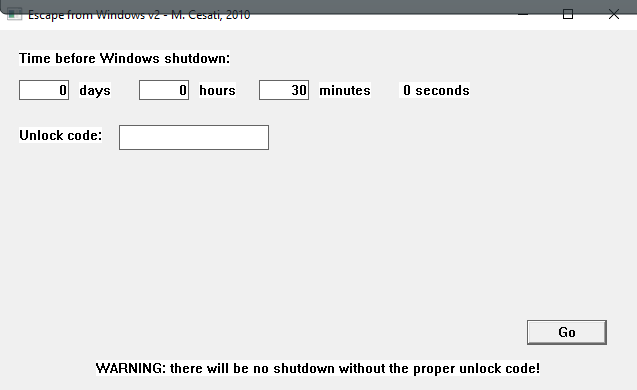
\includegraphics[scale=0.5]{immagini/app1}
\caption{Schermata iniziale dell'applicativo}
\label{Figura 1}
\end{figure}
\vspace{3cm}
\begin{figure}[!h]
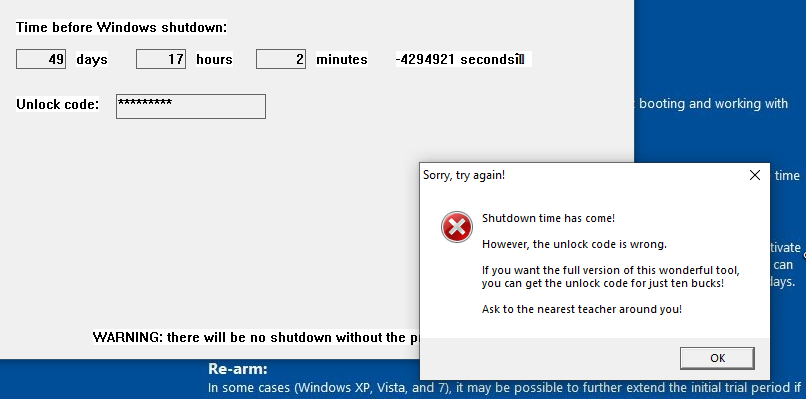
\includegraphics[scale=0.5]{immagini/app2}
\caption{Messaggio di errore}
\label{Figura 2}
\end{figure}
\vspace{3cm}
\begin{figure}[!h]
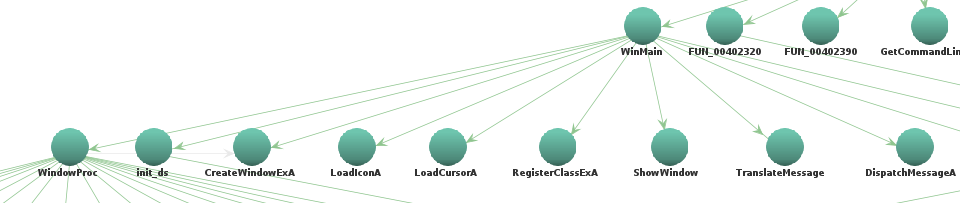
\includegraphics[scale=0.5]{immagini/win_main}
\caption{Ramo dell'albero dove viene chiamato il WinMain}
\label{Figura 3}
\end{figure}
\vspace{3cm}
\begin{figure}[!h]
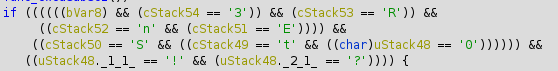
\includegraphics[scale=1]{immagini/sblocco}
\caption{Controllo del valore recuperato dalla GetDlgItemText}
\label{Figura 4}
\end{figure}
\vspace{3cm}
\begin{figure}[!h]
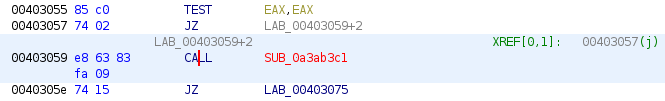
\includegraphics[scale=0.8]{immagini/path}
\\\\
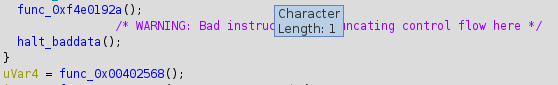
\includegraphics[scale=0.8]{immagini/non_risolto}
\caption{Istruzioni non disassemblate correttamente da Ghidra}
\label{Figura 5}
\end{figure}
\vspace{3cm}
\begin{figure}[!h]
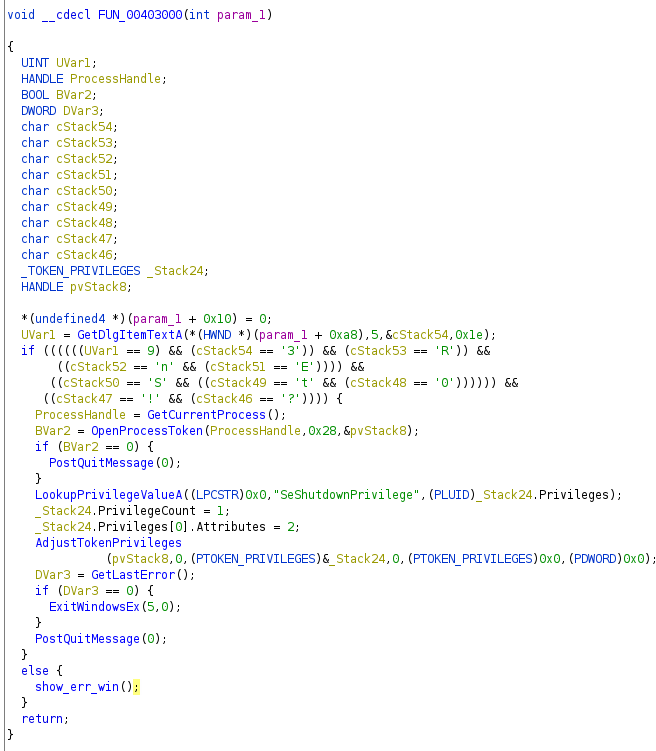
\includegraphics[scale=0.51]{immagini/risolto}
\caption{Risultato della decompilazione}
\label{Figura 6}
\end{figure}








\end{document}